\documentclass[10pt,a4paper,notitlepage,twocolumn]{article}
\usepackage[latin1]{inputenc}
\usepackage{amsmath,amsfonts,amssymb}
\usepackage{graphicx,subfigure}
\usepackage[cm]{fullpage}
\usepackage{url}
\usepackage{stfloats}
%\usepackage{dblfloatfix}
%\usepackage{fixltx2e}

\author{LISA lab, U. of Montreal}
\title{Predicting Network Latency with Graph-Inspired Models}


\begin{document}
\maketitle

\section{Introduction}

This work addresses the problem of predicting the communication latency between two network locations, or addresses, using machine learning techniques.
This task is an essential component of matchmaking applications with minimal latency.
Unlike existing methods that only generalize to unseen pairs from a pool of known addresses, typically by positioning each address in a network map, we also wish to generalize to \emph{unseen addresses}.
%
This task is inherently very noisy and while the obtained relative errors can be as high as 50\%,
our objective for matchmaking purposes is twofold: (1) to correctly predict the order of magnitude of a given connection latency, and (2) to correctly determine the fastest of two candidate connections.

Our basic approach is to model the Internet network as an undirected graph where the shortest distance between two nodes is an estimate of the latency between those locations.
While we could in principle learn both graph connectivity and edge lengths, in this work we will derive connectivity from available geographical information and learn only the edge lengths.

This report extends a previous version from April 22nd, 2013, by Nicolas Boulanger-Lewandowski.

\section{Model}

\subsection{Tree model}

Our basic assumption is that the network topology corresponds to a graph with several interconnected hubs (highly connected nodes) and that the latency between two network locations can be approximated by the distance of the shortest path between two nodes.
Intuitively, the edges will have non-negative weights but this constraint will be lifted later.


\begin{figure}[h]
\centering
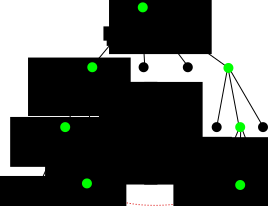
\includegraphics[width=0.8\columnwidth]{../report/tree.pdf}
\caption{The basic graphical model is a tree of depth 3 with edges $l_i\ge0$ representing the latency between network hubs.
The overall latency between two addresses is the distance between two terminal nodes (path in green).
Shortcut edges (red) are added in the extended version.
}
\label{fig:tree}
\end{figure}


In the basic model (Figure~\ref{fig:tree}), we further assume that graph connectivity is known and corresponds to a hierarchy of geographical entities (country, region and city).
Since the resulting graph is a tree, there is a unique path between two nodes and it is easy to learn the edge lengths to minimize the squared error $C$ by solving a non-negative linear system:
\begin{equation} \label{eq:cost}
C \equiv \sum_{j=1}^N(t_j-y_j)^2
\end{equation}
for $N$ training examples with targets $t_j$, $1\le j\le N$ with
\begin{equation} \label{eq:y}
y = M\cdot l
\end{equation}
the predictions of the model and $M_{ji}=1$ if edge $i$ is part of the path linking location pair $j$ and 0 otherwise.

\subsection{Extended model}

We now extend the basic tree model to have the following properties:
\begin{enumerate}
\item It should be possible to add direct edges, or shortcuts, between important hubs to bypass the default hierarchy (e.g., red edge in Figure~\ref{fig:tree}).
\item The prediction should degrade gracefully with sparse data, e.g., a city unseen during training should inherit the average behavior of its parent region or country.
\item The model should also incorporate additional information such as physical distance, connection medium or full IP address.
\item The model should be robust to outliers, in particular unusually long delays.
\end{enumerate}

The strategy is to express the predictions as a regularized sum of $K$
terms with weight decay coefficients $\lambda_k$ and each term will be
chosen to represent an aspect (feature) of the input address pair.
To limit the weight of outliers, we minimize the {\em absolute error},
instead of the squared error used in Equation~\ref{eq:y}\footnote{The
model in the previous report used the squared error, or $L_2$ norm.}.

Equations~(\ref{eq:cost}-\ref{eq:y}) become:
\begin{equation} \label{eq:cost2}
C \equiv \sum_{j=1}^N\left|t_j-y_j\right| + \sum_{k=1}^K \lambda_k \left\|l^{(k)}\right\|^2
\end{equation}
\begin{equation} \label{eq:y2}
y = \sum_{k=1}^K M^{(k)}\cdot l^{(k)}
\end{equation}
where $M_{j:}^{(k)}$ represents the $k$-th feature vector of the $j$-th example, e.g., a one-hot vector representing the city of the host address, a one-hot vector representing the country combination of both addresses, or a real value giving the physical distance between the two locations.
It is easy to see that the basic tree model of Figure~\ref{fig:tree} can be recovered by this framework simply by using $K=7$ terms: \texttt{city1, region1, country1, country2, region2, city2} and a constant.
%
It is also possible to use second-order terms such as \texttt{(country1, country2)} or \texttt{(city1, city2)} to add direct edges in the graph, satisfying requirement 1 above, or other miscellaneous information fulfilling requirement 3 above.

The regularization coefficient $\lambda_k$ will effectively diminish
the salience of a feature rarely present in the data (that could be
spurious) by demanding that each $l_i^{(k)}$ affects a large number
of training examples (equation~\ref{eq:cost2}).  For example, the
correction due to a \texttt{(city1, city2)} term will be weighted by
\begin{equation} \label{eq:regularize}
  (1+\lambda_k/n)^{-1}
\end{equation}
for $n$ occurences of a given city pair during training due to the
regularization.
Since corrections associated with sparse data will tend to be small, the model will naturally fall back to features with a lot of training data (e.g., first-order terms), satisfying requirement 2 above.
It is important not to constrain the $l^{(k)}_i$ to be non-negative in this context because corrections to a coarse predictor may go in either direction.

Minimizing equation~(\ref{eq:cost2}) involves solving a huge sparse
linear system with $N\cdot n_f$ entries, where the number of training
examples $N\simeq 10^6 \text{\ to } 10^8$ and the number of input
features $n_f\simeq10^{10}$ in our experiments.

A more efficient approach is to optimize each successive term $l^{(k)}$ in a greedy fashion by keeping the previous ones fixed, which makes each $M^{(k)}$ in reduced row echelon form and readily invertible.
This greedy approximation becomes exact as $\lambda_k\rightarrow 0$, eliminates the underdetermination associated with subpopulation terms (e.g. \texttt{city1} $\subset$ \texttt{country1}) and helps generalization.
This approach also makes it easier to select the hyperparameters $\lambda_k$ and to adaptively learn the parameters $l^{(k)}$ in an online setting.


\section{Experiments}

\subsection{Error metrics}

In the following experiments, we will report results using the following
metrics, where, for example $j$, $t_j$ is the target (actual measured
delay), and $y_j$ is the predicted delay.

We report {\em $L_1$ and $L_2$ errors:}
\begin{equation}
L_p = \sqrt[p]{\frac1N\sum_{j=1}^N \left|t_j-y_j\right|^p},
\end{equation}
%
the {relative error:}
\begin{equation}
RE = \frac1N\sum_{j=1}^N \frac{|t_j-y_j|}{t_j},
\end{equation}
%
the {\em confusion matrix} $C$:
\begin{equation}
C_{ab} = \sum_{j=1}^N
\begin{cases}
1 & \text{\ if } a=c(t_j),b=c(y_j) \\ 
0 & \text{\ otherwise}
\end{cases},
\end{equation}
where $c(\cdot)$ denotes the class label of a given latency value as defined in Table~\ref{tab:cl_l12},
or the row-normalized version:
\begin{equation}
C'_{ab} = \frac{C_{ab}}{\sum_{b'} C_{ab'}},
\end{equation}
%
the {\em classification accuracy}\/:
\begin{equation}
CA = \frac{\operatorname{Tr}(C)}N.
\end{equation}

We also report a few measurements of {\em ordering accuracy}, where we define
the ordering accuracy for two examples $j$ and $j'$ as:
\begin{equation}
  OA(j, j') =
  \begin{cases}
    1 & \text{\ if } t_j > t_{j'} \text{\ and } y_j > y_{j'} \\
    1 & \text{\ if } t_j < t_{j'} \text{\ and } y_j < y_{j'} \\
    1 & \text{\ if } t_j = t_{j'} \\
    \frac{1}{2} & \text{\ if } t_j \neq t_{j'} \text{\ and } y_j = y_{j'} \\
    0 & \text{\ otherwise.}
  \end{cases}
\label{eq:oa}
\end{equation}
The ordering accuracy corresponds to the probability of choosing
successfully, between two address pairs, which has the smallest
latency, and is an important indicator of the usefulness of a model in
matchmaking applications. When both pairs have exactly the same latency
(third case), we consider both predictions as successes. When both
predictions are the same (fourth case), we use a score of $\frac{1}{2}$,
so the measure is symmetrical\footnote{The previous report used a
slightly different definition of the ordering accuracy.}.

In particular, we will report the ordering accuracy averaged over all
pairs of data:
\begin{equation}
 OA_{\text{Pairs}} =  \frac2{N(N-1)}\sum_{j=1}^N\sum_{j'>j}^N OA(j, j'),
\end{equation}
%
which can also be defined class-wise, i.e., the sum for $OA_{ab}$ being
only over $j,j'$ indices for which $a=c(t_j),b=c(t_{j'})$, and properly
normalized. In practice, to avoid considering all possible pairs,
we estimate this cost by sampling $500,000$ pairs at random.

In order to reflect the need for a matchmaking application to choose the
fastest destination IP for a given source IP, we will also compute the
ordering accuracy of all $(j, j')$ pairs sharing the same source IP, and
report their mean (where each origin IP has the same weight, denoted
``ordering accuracy normalized by source IP'', or ``OA/IP'').

\subsection{Data Sets}
\label{sec:data}

\subsubsection{iOS Games}
\label{sec:data_ios}

The iOS Games data set (or ``iOS'') consists of ICMP round-trip times
between wireless peers (Wi-Fi, 3G or other) collected during iOS games,
from May 2012 to June 2013.

The original data was filtered to remove unsuccessful ping attempts,
duplicates (examples where the origin IP, the destination IP and the
measured delay were exactly the same) and remove examples with delays
greater than 5000~ms, giving \mbox{$N=4,146,598$} examples.
The data, still ordered chronologically, was then
split into training, validation and test sets using a 8:1:1
ratio\footnote{The previous report used data collected until August 2012
only, without filtering out duplicates, and used a random (rather than
chronological) split.}.

\subsubsection{Assassin's Creed}

The ``Assassin's Creed'' (or ``AC'') data set is composed of data
collected from two games: {\em Assassin's Creed Revelations}\ 
($2,086,908$ samples collected between November 2011 and March 2013)
and {\em Assassin's Creed III}\ ($1,439,458$ samples collected between
October 2012 and March 2013).

Each of these samples contain ping measurements from both ends of the
connection. After creating two training samples for each of the original
samples (one for each direction) and removing duplicates, the data from
each source was split independently into training, validation and test
using the same 8:1:1 ratio. These sets are then combined to form the
final training, validation and test set, for a total of $N=6,533,214$
examples.

\subsubsection{Internet Census 2012 ICMP}

This data set was extracted from the Internet Census 2012 ICMP Ping
data\footnote{\url{http://internetcensus2012.bitbucket.org/download.html}},
collected from compromised embedded systems on the Internet (for
instance, routers).

Only the successful attempts with a delay of 5000 ms or less were kept.
The $N=74,679,517$ samples were ordered chronologically, and split
between training, validation, and test sets with a 8:1:1 ratio.

\subsection{Baseline Models}

We compare our graphical model to other baselines:
\begin{itemize}
  \item a constant prediction,
  \item a linear regression on the physical distance obtained
via IP2Location, and
  \item predicting the average latency between the two
communicating countries.
\end{itemize}


\section{Results}

\subsection{Absolute and Relative Errors}

\begin{table*}[htp]
\centering
\begin{tabular}{|rrrl|}
\hline \multicolumn{3}{|c}{$L_1$ (ms)} & Added Term \\
iOS & AC & IC2012 &  \\ \hline\hline
169.4 & 71.3 & 120.0 & constant \\
155.4 & 55.3 & 120.0 & distance \\
155.4 & 55.3 & 120.0 & type1 \\
155.4 & 55.3 & 120.0 & type2 \\
155.4 & 55.3 & 120.0 & (type1, type2) \\
141.4 & 53.8 & 91.9 & country1 \\
133.5 & 53.5 & 91.8 & country2 \\
133.1 & 53.0 & 91.8 & same\_country \\
127.1 & 50.4 & 91.5 & (country1, country2) \\
127.1 & 50.4 & 91.5 & (country1, country2, type1, type2) \\
126.4 & 50.1 & 90.1 & region1 \\
126.2 & 50.1 & 89.6 & region2 \\
126.1 & 49.8 & 89.6 & same\_region \\
125.3 & 49.8 & 89.3 & (region1, region2) \\
125.2 & 49.7 & 88.8 & city1 \\
125.0 & 49.7 & 88.7 & city2 \\
125.0 & 49.3 & 88.7 & same\_city \\
125.0 & 49.4 & 88.3 & (city1, city2) \\
124.9 & 49.4 & 84.7 & ip1 \\
124.7 & 49.4 & 84.7 & ip2 \\
124.7 & 49.4 & - & (ip1, ip2) \\
\hline
\end{tabular}
\caption{Evolution of the test $L_1$ error with each term added to our
graphical model, for the different data sets used.}
\label{tab:terms}
\end{table*}

Table~\ref{tab:terms} shows the $K=21$ terms we have retained in our
extended model, and their contribution to the test $L_1$ error,
on the different data sets.  For each term, $\lambda_k$
is chosen so as to optimize the validation $L_1$ error using the
downhill simplex algorithm with initial value $\lambda_{k0}=10$.

Due to the large size of the Internet Census 2012 data set, it was not
possible to perform the regression using the \texttt{(ip1, ip2)} pairs.


\begin{table*}[htp]
\centering
\begin{tabular}{|l|c|c|c|c|c|c|}
\hline Model & $L_1$ (ms)  & $L_2$ (ms) & Rel Err & Class Acc & OA/Pairs & OA/IP \\ \hline\hline
Constant prediction & 169.4 & 283.7 & 68.3\% & 31.3\% & 50.1\% & 50.1\% \\
IP2Location         & 155.4 & 283.4 & 62.8\% & 33.1\% & 65.4\% & 62.0\% \\
Country pairs       & 127.9 & 268.5 & 51.7\% & 52.0\% & 74.4\% & 68.5\% \\
Graphical model & \bf 124.7 & \bf 264.8 & \bf 50.5\% & \bf 54.0\% & \bf 75.7\% & \bf 69.3\% \\ \hline 
\end{tabular} 
\caption{Prediction performance on the iOS data set, compared with the baseline models.}
\label{tab:comp_ios}
\end{table*}

\begin{table*}[htp]
\centering
\begin{tabular}{|l|c|c|c|c|c|c|}
\hline Model & $L_1$ (ms)  & $L_2$ (ms) & Rel Err & Class Acc & OA/Pairs & OA/IP \\ \hline\hline
Constant prediction & 71.3 & 133.3 & 59.4\% & 49.0\% & 50.2\% & 50.4\% \\
IP2Location         & 55.3 & 117.2 & 46.0\% & 53.0\% & 73.7\% & 66.9\% \\
Country pairs       & 54.2 & 117.2 & 45.2\% & 54.4\% & 69.2\% & 64.0\% \\
Graphical model & \bf 49.4 & \bf 112.9 & \bf 41.1\% & \bf 61.2\% & \bf 74.8\% & \bf 68.2\% \\ \hline 
\end{tabular} 
\caption{Prediction performance on the Assassin's Creed data set, compared with the baseline models.}
\label{tab:comp_ac}
\end{table*}

\begin{table*}[htp]
\centering
\begin{tabular}{|l|c|c|c|c|c|c|}
\hline Model & $L_1$ (ms)  & $L_2$ (ms) & Rel Err & Class Acc & OA/Pairs & OA/IP \\ \hline\hline
Constant prediction & 120.1 & 172.5 & 67.2\% & 25.6\% & 50.1\% & 50.4\% \\
IP2Location         & 120.1 & 172.5 & 67.1\% & 25.6\% & 51.3\% & 50.4\% \\
Country pairs       &  91.4 & 151.8 & 51.1\% & 51.6\% & 72.1\% & 50.4\% \\
Graphical model & \bf 84.7 & \bf 143.8 & \bf 47.4\% & \bf 53.5\% & \bf 74.7\% & 50.4\% \\ \hline 
\end{tabular} 
\caption{Prediction performance on the Internet Census 2012 data set, compared with the baseline models.}
\label{tab:comp_ic2012}
\end{table*}


Tables~\ref{tab:comp_ios} to~\ref{tab:comp_ic2012} present the
performance of the evaluated models in the latency prediction task on
the different data sets described in Section~\ref{sec:data}.
The proposed model clearly outperforms other baselines on all data sets.

While the obtained $L_{1,2}$ and relative errors remain relatively high,
the classification accuracy (53.5\% to 61.2\%) and ordering accuracy
between all pairs (around 75\%)
indicate that the graphical model predictions lie in a reasonable range
and suffice to determine the fastest of two addresses in the majority of
cases.

The ordering accuracy normalized by IP is lower than when it is computed
among all pairs, but still reasonable on iOS (69.3\%) and Assassin's
Creed (68.2\%), but surprisingly low (50.4\%, with no discriminative
power) on IC2012.  Further measurements and analysis of ordering
accuracy are presented in Section~\ref{sec:oa}.

\subsection{Latency Classes and Confusion Matrix}
\begin{table*}[ht]
\centering
\begin{tabular}{|cc|cc|cc|cc|}
\hline
      &            & \multicolumn{2}{c|}{iOS} & \multicolumn{2}{c|}{AC} & \multicolumn{2}{c|}{IC2012} \\
Class & Range (ms) & $L_1$ (ms) & $L_2$ (ms) & $L_1$ (ms) & $L_2$ (ms) & $L_1$ (ms) & $L_2$ (ms) \\ \hline\hline
1 & 0--99      & 124.4 & 266.8 & 49.4 & 114.5 & 84.7 & 144.4 \\
2 & 100--199   & 125.1 & 266.7 & 49.5 & 114.1 & 84.5 & 143.5 \\
3 & 200--299   & 125.0 & 266.2 & 49.3 & 106.9 & 84.7 & 143.7 \\
4 & 300--499   & 124.7 & 264.6 & 48.7 & 110.5 & 84.7 & 144.0 \\
5 & 500--999   & 123.9 & 260.1 & 50.5 & 103.8 & 84.9 & 143.4 \\
6 & 1000--5000 & 121.8 & 259.4 & 49.5 & 110.7 & 84.9 & 141.9 \\
\hline
\end{tabular}
\caption{Definition of the latency classes and their associated $L_1$ and $L_2$ errors.}
\label{tab:cl_l12}
\end{table*}


Table~\ref{tab:cl_l12} indicates the ranges used to define the latency
classes.  Surprisingly, the $L_1$ and $L_2$ errors do not vary much with
the magnitude of the target. This effect is consistent across all three
data sets.  This could indicate an intrinsic noise to the measurement
process that is added to a more deterministic network-specific baseline
latency.


\begin{figure*}[ht]
\centering
\subfigure[iOS Games]{\includegraphics[width=0.75\columnwidth]{figures/iOS_full_LAD_confusion.pdf}}
\subfigure[Assassin's Creed]{\includegraphics[width=0.75\columnwidth]{figures/AC_full_LAD_confusion.pdf}}
\subfigure[Internet Census 2012]{\includegraphics[width=0.75\columnwidth]{figures/IC2012_full_LAD_confusion.pdf}}
\caption{Row-normalized confusion matrices $C'_{ab}$ (row: target class $c(t_j)$, column: predicted class $c(y_j)$).}
\label{fig:conf}
\end{figure*}


The ability of the graphical model to correctly identify the order of
magnitude of latency can also be measured in the confusion matrix,
displayed in Figure~\ref{fig:conf}.  The model is able to capture the
correlation, especially for classes 2 to 4, on all data sets. Really
small values (class 1, less than 100 ms), however, are usually predicted
as class 2. The same phenomenon arises for larger values: classes 5 and
6 are often mapped to class 4.  However, these classes represent a small
proportion of the data, and it is possible that most of the large values
are outlier values for two addresses that usually have a more reasonable
delay. This would also explain why the confusion matrix is worse on the
Assassin's Creed data set, as most of its data consists of class 2, and
even classes 3 and 4 have a really small number of examples.

\subsection{Ordering Accuracy}
\label{sec:oa}

\begin{figure*}[p]
\centering
\subfigure[Constant prediction, OA]{\includegraphics[width=0.75\columnwidth]{figures/iOS_constant_LAD_oa_5000ms}}
\subfigure[Constant prediction, OA/IP]{\includegraphics[width=0.75\columnwidth]{figures/iOS_constant_LAD_oaip_5000ms_skip}}
\subfigure[IP2Location, OA]{\includegraphics[width=0.75\columnwidth]{figures/iOS_distance_LAD_oa_5000ms}}
\subfigure[IP2Location, OA/IP]{\includegraphics[width=0.75\columnwidth]{figures/iOS_distance_LAD_oaip_5000ms_skip}}
\subfigure[Country pairs, OA]{\includegraphics[width=0.75\columnwidth]{figures/iOS_countries_LAD_oa_5000ms}}
\subfigure[Country pairs, OA/IP]{\includegraphics[width=0.75\columnwidth]{figures/iOS_countries_LAD_oaip_5000ms_skip}}
\subfigure[Graphical model, OA]{\includegraphics[width=0.75\columnwidth]{figures/iOS_full_LAD_oa_5000ms}}
\subfigure[Graphical model, OA/IP]{\includegraphics[width=0.75\columnwidth]{figures/iOS_full_LAD_oaip_5000ms_skip}}
\caption{Ordering accuracy (blue curve) between pairs of examples from the {\bf
iOS Games} test set, considering only pairs for which the difference
in delays is over some threshold. That threshold corresponds to the
x axis. The gray curve shows the proportion of data actually
considered.}
\label{fig:oa_ios}
\end{figure*}

\begin{figure*}[p]
\centering
\subfigure[Constant prediction, OA]{\includegraphics[width=0.75\columnwidth]{figures/AC_constant_LAD_oa_5000ms}}
\subfigure[Constant prediction, OA/IP]{\includegraphics[width=0.75\columnwidth]{figures/AC_constant_LAD_oaip_5000ms_skip}}
\subfigure[IP2Location, OA]{\includegraphics[width=0.75\columnwidth]{figures/AC_distance_LAD_oa_5000ms}}
\subfigure[IP2Location, OA/IP]{\includegraphics[width=0.75\columnwidth]{figures/AC_distance_LAD_oaip_5000ms_skip}}
\subfigure[Country pairs, OA]{\includegraphics[width=0.75\columnwidth]{figures/AC_countries_LAD_oa_5000ms}}
\subfigure[Country pairs, OA/IP]{\includegraphics[width=0.75\columnwidth]{figures/AC_countries_LAD_oaip_5000ms_skip}}
\subfigure[Graphical model, OA]{\includegraphics[width=0.75\columnwidth]{figures/AC_full_LAD_oa_5000ms}}
\subfigure[Graphical model, OA/IP]{\includegraphics[width=0.75\columnwidth]{figures/AC_full_LAD_oaip_5000ms_skip}}
\caption{Ordering accuracy (blue curve) between pairs of examples from the {\bf
Assassin's Creed} test set, considering only pairs for which the difference
in delays is over some threshold. That threshold corresponds to the
x axis. The gray curve shows the proportion of data actually
considered.}
\label{fig:oa_ac}
\end{figure*}

\begin{figure*}[p]
\centering
\subfigure[Constant prediction, OA]{\includegraphics[width=0.75\columnwidth]{figures/IC2012_constant_LAD_oa_5000ms}}
\subfigure[Constant prediction, OA/IP]{\includegraphics[width=0.75\columnwidth]{figures/IC2012_constant_LAD_oaip_5000ms_skip}}
\subfigure[IP2Location, OA]{\includegraphics[width=0.75\columnwidth]{figures/IC2012_distance_LAD_oa_5000ms}}
\subfigure[IP2Location, OA/IP]{\includegraphics[width=0.75\columnwidth]{figures/IC2012_distance_LAD_oaip_5000ms_skip}}
\subfigure[Country pairs, OA]{\includegraphics[width=0.75\columnwidth]{figures/IC2012_countries_LAD_oa_5000ms}}
\subfigure[Country pairs, OA/IP]{\includegraphics[width=0.75\columnwidth]{figures/IC2012_countries_LAD_oaip_5000ms_skip}}
\subfigure[Graphical model, OA]{\includegraphics[width=0.75\columnwidth]{figures/IC2012_full_LAD_oa_5000ms}}
\subfigure[Graphical model, OA/IP]{\includegraphics[width=0.75\columnwidth]{figures/IC2012_full_LAD_oaip_5000ms_skip}}
\caption{Ordering accuracy (blue curve) between pairs of examples from the {\bf
Internet Census 2012} test set, considering only pairs for which the difference
in delays is over some threshold. That threshold corresponds to the
x axis. The gray curve shows the proportion of data actually
considered.}
\label{fig:oa_ic2012}
\end{figure*}

In a matchmaking scenario, it is more important to be able to
discriminate between latency pairs when the difference between both
is bigger: a difference of a few milliseconds does not matter as
much.  Figures~\ref{fig:oa_ios} to~\ref{fig:oa_ic2012} show the
ordering accuracy when we only consider pairs of test examples where
the difference in targets is bigger than some threshold. The different
thresholds used are used as the x axis. Figures on the left show the
ordering accuracy between random pairs, figures on the right show
the ordering accuracy normalized by source IP.

The peak for a threshold of 0, observed in particular for the constant
predictor (bringing their accuracy to more than 50\%) is due to fact
that we consider both predictions correct when the targets are equal
(case 4 of Equation~\ref{eq:oa}), which cannot happen when there
is a minimal delay.

As we already saw in Tables~\ref{tab:comp_ios} to~\ref{tab:comp_ic2012},
the ordering accuracy normalized by source IP is lower than when
considering all pairs.
One explanation for that is that this task is harder,
because for each comparison, the origin IP is the same, so none of the
factors related to the source only (\texttt{type1}, \texttt{country1},
etc.) are actually useful. This is consistent with the fact that, on
IC2012, where this effect is the strongest, these are the only factors
that contribute significantly to the minimization of the $L_1$ error (see
Table~\ref{tab:terms}).


\subsection{Qualitative Assessments}

\begin{figure*}[htb]
\centering
\subfigure[iOS Games]{\includegraphics[width=0.75\columnwidth]{figures/iOS_full_LAD_scatter.pdf}}
\subfigure[Assassin's Creed]{\includegraphics[width=0.75\columnwidth]{figures/AC_full_LAD_scatter.pdf}}
\subfigure[Internet Census 2012]{\includegraphics[width=0.75\columnwidth]{figures/IC2012_full_LAD_scatter.pdf}}
\caption{A few targets and predictions by the graphical model randomly
chosen from the different test sets.}
\label{fig:samples}
\end{figure*}


A qualitative assessment of the model performance and predictions can
be obtained by plotting a few predictions randomly chosen from the test
set (Figure~\ref{fig:samples}).  Again, the model correctly predicts the
order of magnitude of the latency most of the time. We also see, on the
right side of these plots, the distribution of higher-latency samples,
that seem to be distributed randomly, regardless of the prediction.

Finally, plots showing the correlation of the targets with the
predictions of different models can be found in Figures~\ref{fig:ios_2d}
to~\ref{fig:ic2012_2d}.

%Finally, detailed error distributions that further highlight the
%advantage of our model are presented in Appendix~\ref{app:error_distr}.


\subsection{Other Considerations}

When performing preliminary experiments, which are not thoroughly
reported here, we came across the following conclusions, that can be
important to keep in mind when collecting data and using this model.

The GeoIP data associated to an IP can
change over time. For instance, the GeoLite
Database\footnote{\url{http://dev.maxmind.com/geoip/legacy/geolite/}}
reports a loss of accuracy of 1.5\% each month.  Therefore, it is
important to extract the GeoIP data (coordinates, country, region, and
city) using a recent version of the data base, as soon as the data is
collected.  For the experiments presented here, the GeoIP data was not
collected along with the IPs and delays, so we used a recent version of
the GeoIP data, even for older data.

To investigate the bad performance of the IP2Location distance as a
predictor on the iOS data set, we trained the different models on a
subset of data, containing only Wi-Fi to Wi-Fi connection (excluding
cellular connections at source and destination). The results were not
significantly different from the ones using the whole data set, and were
not reported here.

To try and explain why the ordering accuracy by IP gives bad
performances (50.4\%, the same as the constant predictor) on the
Internet Census 2012 data, we hypothesized that difference in the
relative weights of examples played a role. For instance, if an IP is
present as a source IP in a data set $10,000$ times more often than
another one, then it will have a relative weight $10,000$ higher in the
training phase, but the OA/IP will give the same weight to both. Instead
of the simple average, we also computed a weighted average where each
source IP is given a weight relative to its frequency in the test
test. These weighted average have values similar to the un-weighted ones,
and are not reported here.

Among the data sets used, iOS is the one wich resembles most the context
in which a matchmaking predictor would take place, for two reasons.
First, all the device participating in the data collection (source and
destination of the ping) are devices used for gaming at that time, in
contrast to IC2012, where source devices are compromised system all over
the Internet, and destinations are random IPs. Second, these devices
are not necessarily playing with each other, whereas Assassin's Creed
data is biased by the fact that the two players are actually connected
to each other, which may not have been the case if the latency was too
high.

\section{Conclusion}

We have proposed a graph-inspired model to predict the communication
latency between pairs of unseen network addresses.  The model obtained a
test classification accuracy over 50\% on all data sets, and the $L_1$
error showing low variability across all ranges indicates an accurate
prediction of the latency order of magnitude.

This ability translates into a high ordering accuracy (around 75\% on
all data sets).  The model is also able to discriminate fairly well
between two candidate pairs with the same origin IP on data coming
from games (OA/IP around 70\% for iOS and Assassin's Creed), which
is sufficiently useful to discern between candidate connections in
matchmaking applications.

The proposed model outperforms IP2Location on all tested data sets,
for a variety of metrics. On the iOS Games data set, which seems most
relevant for the task of matchmaking, the global ordering accuracy is
largely better (75.7\% compared to 65.4\%), as well as the ordering
accuracy by origin IP (69.3\% vs. 62.0\%).

On the Assassin's Creed data set, for which the players already have a
low latency, the gain of the graphical model compared to IP2Location is
lower (74.8\% vs. 73.7\% in global ordering accuracy, 68.2\% vs. 66.9\%
normalized by source IP), but still consistent across measures.

For the Internet Census 2012 data set, the graph-inspired model also
outperforms IP2Location for all metrics (74.7\% in ordering accuracy
vs. 51.3\%), except for the discriminating ordering accuracy by origin
IP, where no model was able to get better than a random prediction,
probably because the distribution of training examples was quite different
from the distribution we expect in a matchmaking task.


\clearpage
\appendix
%\section{Prediction distributions}
\label{app:error_distr}

\iffalse
\begin{figure*}[!h]
\centering
\subfigure[Constant prediction]{\includegraphics[width=0.75\columnwidth]{figures/iOS_constant_LAD_dist}}
\subfigure[IP2Location]{\includegraphics[width=0.75\columnwidth]{figures/iOS_distance_LAD_dist}}
\subfigure[Country pairs]{\includegraphics[width=0.75\columnwidth]{figures/iOS_countries_LAD_dist}}
\subfigure[Graphical model]{\includegraphics[width=0.75\columnwidth]{figures/iOS_full_LAD_dist}}
\caption{Distribution of the test error $(t_j-y_j)$ on the iOS data set.}
\label{fig:ios_dist}
\end{figure*}

\begin{figure*}[!h]
\centering
\subfigure[Constant prediction]{\includegraphics[width=0.75\columnwidth]{figures/iOS_constant_LAD_rdist}}
\subfigure[IP2Location]{\includegraphics[width=0.75\columnwidth]{figures/iOS_distance_LAD_rdist}}
\subfigure[Country pairs]{\includegraphics[width=0.75\columnwidth]{figures/iOS_countries_LAD_rdist}}
\subfigure[Graphical model]{\includegraphics[width=0.75\columnwidth]{figures/iOS_full_LAD_rdist}}
\caption{Distribution of the test relative error $|t_j-y_j|/t_j$ on the iOS data set.}
\label{fig:ios_rdist}
\end{figure*}

\fi

\begin{figure*}
\centering
\subfigure[Constant prediction]{\includegraphics[width=0.75\columnwidth]{figures/iOS_constant_LAD_2d}}
\subfigure[IP2Location]{\includegraphics[width=0.75\columnwidth]{figures/iOS_distance_LAD_2d}}
\subfigure[Country pairs]{\includegraphics[width=0.75\columnwidth]{figures/iOS_countries_LAD_2d}}
\subfigure[Graphical model]{\includegraphics[width=0.75\columnwidth]{figures/iOS_full_LAD_2d}}
\caption{Heat map of the test joint distribution $P(t_j,y_j)$ estimated with a Gaussian kernel ($\sigma=18$~ms) on the {\bf iOS games} data set.}
\label{fig:ios_2d}
\end{figure*}

\begin{figure*}
\centering
\subfigure[Constant prediction]{\includegraphics[width=0.75\columnwidth]{figures/AC_constant_LAD_2d}}
\subfigure[IP2Location]{\includegraphics[width=0.75\columnwidth]{figures/AC_distance_LAD_2d}}
\subfigure[Country pairs]{\includegraphics[width=0.75\columnwidth]{figures/AC_countries_LAD_2d}}
\subfigure[Graphical model]{\includegraphics[width=0.75\columnwidth]{figures/AC_full_LAD_2d}}
\caption{Heat map of the test joint distribution $P(t_j,y_j)$ estimated with a Gaussian kernel ($\sigma=18$~ms) on the {\bf Assassin's Creed} data set.}
\label{fig:ac_2d}
\end{figure*}

\begin{figure*}
\centering
\subfigure[Constant prediction]{\includegraphics[width=0.75\columnwidth]{figures/IC2012_constant_LAD_2d}}
\subfigure[IP2Location]{\includegraphics[width=0.75\columnwidth]{figures/IC2012_distance_LAD_2d}}
\subfigure[Country pairs]{\includegraphics[width=0.75\columnwidth]{figures/IC2012_countries_LAD_2d}}
\subfigure[Graphical model]{\includegraphics[width=0.75\columnwidth]{figures/IC2012_full_LAD_2d}}
\caption{Heat map of the test joint distribution $P(t_j,y_j)$ estimated with a Gaussian kernel ($\sigma=18$~ms) on the {\bf Internet Census 2012} data set.}
\label{fig:ic2012_2d}
\end{figure*}

\section{Code and Saved Model}

The code to train and load the graphical model
is available in the ``pings'' repository on
GitHub\footnote{\url{https://github.com/lisa-lab/pings}}. The code
for training the model and retrieving its predictions is in
\verb|models/work_in_progress/src/graph.py|. It was tested with the following
version of its dependencies:
\begin{itemize}
  \item Python 2.7.2
  \item NumPy 1.6.1
  \item SciPy 0.9.0.
\end{itemize}
The GeoLite GeoIP data base was retrieved in May 2013.

After training, the model parameters are saved in a pickle file with
the following structure. The file contains a pair
\verb|(saved_params, terms)|, where \verb|terms| is a list of the terms
used in the model, as described in Table~\ref{tab:terms}. For each term
in that list, the last value represents the regularization penalty
used; it will be 0 for the constant term or bias, and for the GeoIP
distance, and -1 for all other terms, meaning it should be optimized on
the validation set.

\verb|saved_params| is a list of the same length, each element of
that list is a triplet containing the data necessary to compute the
contribution of that term. There are 3 possible cases:
\begin{itemize}

  \item If the term is a real value, which is only the case for
  the distance, the triplet contains \verb|(coef, bias, reg)|,
  where \verb|coef| is the coefficient of the linear regression,
  \verb|bias| is the bias, and \verb|reg| is the regularization
  coefficient (similar to the one described in Equations~\ref{eq:cost2}
  and~\ref{eq:regularize}, except no division by $n$ would occur).
  so the final contribution of that term in the prediction is:
  \begin{equation}
    M^{(k)}_{j,:} \cdot \frac{\mathtt{coeff}}{1 + \mathtt{reg}} + \mathtt{bias}.
  \end{equation}

  \item If the term is a one-hot vector with fewer than 2000 possible
  classes (for instance, the connection type \verb|type1|),
  the triplet contains \verb|(params, number, reg)|, where \verb|params|
  and \verb|numbers| are NumPy \verb|ndarray| vectors, with their length
  equal to the number of possible classes, containing respectively the
  regression coefficients and the training example count for each of the
  possible input classes.
  \verb|reg| is the coefficient $\lambda_k$, as described in Equations~\ref{eq:cost2}
  and~\ref{eq:regularize}, so the final contribution of that term
  in the prediction is:
  \begin{equation}
    M^{(k)}_{j,:} \cdot \frac{\mathtt{params}}{1 + \mathtt{reg} / \mathtt{numbers}},
  \end{equation}
  where all divisions are done element-wise.
  Note that, if $M^{(k)}_{j,:}$ is a one-hot vector where $M^{(k)}_{j,i} = 1$,
  this is equivalent to the scalar:
  \begin{equation}
    \frac{\mathtt{params}_i}{1 + \mathtt{reg} / \mathtt{numbers}_i}.
  \end{equation}

  \item If the term would be represented by a one-hot vector with 2000
  classes or more (for instance, the source IP \verb|ip1|), the triplet
  is also \verb|(params, number, reg)|, but a dictionary structure (more
  precisely, a Python \verb|collections.defaultdict|) is used to store
  the coefficients (\verb|params|) and counts (\verb|numbers|) instead.
  If the $k$-th feature of example $j$ is the class $i$, the contribution
  of that term to the prediction is:
  \begin{equation}
    \frac{\mathtt{params[i]}}{1 + \mathtt{reg} / \mathtt{numbers[i]}},
  \end{equation}
  where \verb|d[i]| denotes the value of dictionary \verb|d| associated
  to key \verb|i|, or 0 if \verb|i| is not a key of \verb|d|.

\end{itemize}

\end{document}
